\chapter{Méthodologie d'analyse}\label{cap:methodologie}
%--------------------------------------

\section{Démarche documentaire}

L'état de l'art a été construit à partir de trois types de sources. Les sources académiques servent à comprendre les concepts : agents LLM, raisonnement avec outils, génération augmentée par récupération, mémoire, collaboration multi-agents et modèles factoriels. Les sources réglementaires servent à fixer les contraintes minimales d'un contexte financier : contrôle du trading algorithmique, résilience opérationnelle, gouvernance du risque IA et auditabilité. Enfin, les dépôts GitHub servent à identifier les solutions réellement disponibles et leur degré de maturité. Lorsque les documents étaient librement accessibles en PDF, ils ont été archivés dans le sous-dossier \texttt{papers} afin de constituer un corpus documentaire local. Les articles soumis à licence éditeur restent cités en bibliographie sans copie locale.

La recherche GitHub a été structurée autour de mots-clés : \emph{LLM agent trading}, \emph{multi-agent financial trading}, \emph{financial LLM agent}, \emph{quantitative trading framework}, \emph{backtesting engine}, \emph{FinRL}, \emph{Qlib}, \emph{OpenBB}, \emph{LangGraph}, \emph{AutoGen} et \emph{CrewAI}. Les dépôts retenus devaient satisfaire au moins l'un des critères suivants :

\begin{itemize}
    \item fournir une brique d'orchestration agentique ;
    \item traiter explicitement un cas d'usage financier ;
    \item fournir une infrastructure utile au trading multifactoriel : données, backtesting, moteur d'exécution simulée, apprentissage par renforcement ou recherche quantitative ;
    \item rendre le code accessible publiquement pour étude, adaptation ou expérimentation.
\end{itemize}

Le corpus de comparaison comprend 17 fiches : 6 frameworks généralistes, 6 briques quantitatives et 5 projets spécifiquement financiers. Huit dépôts ont ensuite été retenus pour la due diligence finale, tandis que les autres ont été conservés comme références comparatives ou écartés du prototype. Ce décompte porte sur les fiches étudiées et non sur une mesure exhaustive de tous les dépôts repérés. Les dépôts trop éloignés du sujet, purement marketing, sans code exploitable ou uniquement centrés sur des signaux isolés ont été écartés. Les informations sur GitHub doivent être réévaluées avant toute mise en production, car l'activité, la licence, les dépendances et les mainteneurs peuvent évoluer rapidement.

\section{Revue réglementaire arrêtée au 30 août 2026}

Cette revue est documentaire et ne constitue pas un avis juridique. Elle sert à relier l'architecture proposée aux sources officielles disponibles à la date d'arrêté.

\begin{itemize}
    \item \textbf{MiFID II, article 17 :} le trading algorithmique implique des systèmes et contrôles de risque adaptés, des limites, des tests et une capacité à décrire les paramètres et contrôles à l'autorité compétente \citep{mifidArticle17}.
    \item \textbf{DORA :} le règlement (UE) 2022/2554 s'applique depuis le 17 janvier 2025 et renforce la résilience opérationnelle numérique des entités financières \citep{dora2022}.
    \item \textbf{AI Act :} le règlement (UE) 2024/1689 s'applique en principe depuis le 2 août 2026, avec des dates spécifiques pour certaines dispositions, notamment le 2 février 2025, le 2 août 2025 et le 2 août 2027 \citep{euAiAct2024}. L'applicabilité à un système donné dépend de son usage et de son rôle juridique.
    \item \textbf{NIST AI RMF :} le référentiel AI RMF 1.0 fournit une base de gouvernance, de cartographie, de mesure et de gestion des risques ; la page officielle indique qu'une révision est en cours \citep{nistAirmf2023}.
\end{itemize}

La conséquence opérationnelle est claire : toute mise en production requiert une validation séparée par les fonctions risque, conformité, juridique et IT. Les références ci-dessus doivent être relues à chaque changement de périmètre, de modèle, de fournisseur ou de régime réglementaire.

\section{Grille d'évaluation et scoring}

La grille compare les solutions sans confondre popularité open source et aptitude à un environnement de marché régulé. Chaque critère reçoit une note de 0 à 3 :

\begin{itemize}
    \item 0 : critère absent ou impossible à vérifier dans les sources publiques ;
    \item 1 : élément partiel, seulement illustré ou nécessitant un développement important ;
    \item 2 : capacité documentée et utilisable avec une adaptation maîtrisée ;
    \item 3 : capacité explicite, testable et directement intégrable dans un workflow contrôlé.
\end{itemize}

\begin{table}[H]
\centering
\caption{Grille de scoring des solutions agentiques et quantitatives.}
\label{tab:grille-evaluation}
\scriptsize
\begin{adjustbox}{width=\textwidth}
\begin{tabular}{p{0.18\textwidth}p{0.31\textwidth}p{0.27\textwidth}p{0.18\textwidth}}
\toprule
\textbf{Critère} & \textbf{Question d'évaluation} & \textbf{Barème 0-3} & \textbf{Interprétation} \\
\midrule
Couverture fonctionnelle & Le projet couvre-t-il orchestration, données, backtest, risque, exécution ou reporting ? & 0 absent ; 1 partiel ; 2 plusieurs fonctions ; 3 chaîne cohérente & Mesure l'étendue, sans assimiler étendue et maturité. \\
Reproductibilité & Les calculs et décisions peuvent-ils être rejoués avec les mêmes données et paramètres ? & 0 non vérifiable ; 1 exemples ; 2 pipeline documenté ; 3 tests et versionnement & Condition de base pour audit et validation. \\
Explicabilité & Les sorties relient-elles la justification aux signaux, sources et contraintes ? & 0 aucune ; 1 texte libre ; 2 sorties structurées ; 3 preuve liée aux données & Distingue une narration plausible d'une explication vérifiable. \\
Contrôle du risque & Existe-t-il des limites, validations, stress tests ou garde-fous ? & 0 absent ; 1 implicite ; 2 documenté ; 3 bloquant et testé & Critère critique avant toute exécution. \\
Qualité logicielle & Le dépôt propose-t-il documentation, tests, exemples et structure maintenable ? & 0 absent ; 1 incomplet ; 2 présent ; 3 intégré et suivi & Réduit le risque opérationnel. \\
Intégrabilité & Le projet s'interface-t-il avec Python, bases, API ou moteurs de backtesting ? & 0 isolé ; 1 adaptation forte ; 2 interfaces disponibles ; 3 intégration directe & Détermine la faisabilité d'une architecture composée. \\
Gouvernance & Les rôles, permissions, journaux et validations sont-ils explicitement modélisés ? & 0 absent ; 1 déclaratif ; 2 partiel ; 3 contrôlable et auditable & Indispensable dans une institution financière. \\
\bottomrule
\end{tabular}
\end{adjustbox}
\end{table}

Le score maximal est de 21 points. Les notes ci-dessous sont une lecture documentaire provisoire des dépôts retenus ; elles ne constituent ni une certification, ni une validation de production. Elles servent à rendre visibles les arbitrages effectués dans le mémoire.

\begin{table}[H]
\centering
\caption{Scoring documentaire provisoire des dépôts retenus.}
\label{tab:scoring-depots}
\scriptsize
\begin{adjustbox}{width=\textwidth}
\begin{tabular}{lrrrrrrrr}
\toprule
\textbf{Dépôt} & \textbf{Couverture} & \textbf{Reprod.} & \textbf{Explic.} & \textbf{Risque} & \textbf{Qualité} & \textbf{Intégr.} & \textbf{Gouv.} & \textbf{Total} \\
\midrule
LangGraph & 2 & 3 & 2 & 1 & 3 & 3 & 2 & 16/21 \\
Qlib & 3 & 3 & 1 & 1 & 3 & 3 & 1 & 15/21 \\
Lean & 3 & 3 & 1 & 2 & 3 & 3 & 1 & 16/21 \\
OpenBB & 2 & 2 & 1 & 0 & 3 & 3 & 1 & 12/21 \\
TradingAgents & 2 & 1 & 2 & 0 & 2 & 2 & 1 & 10/21 \\
FinRobot & 2 & 1 & 2 & 0 & 2 & 2 & 1 & 10/21 \\
FinRL & 2 & 2 & 1 & 1 & 2 & 2 & 1 & 11/21 \\
Freqtrade & 3 & 2 & 1 & 1 & 3 & 3 & 1 & 14/21 \\
\bottomrule
\end{tabular}
\end{adjustbox}
\end{table}

Le tableau confirme le choix d'une architecture composée. LangGraph obtient son meilleur niveau sur l'orchestration et l'intégrabilité, tandis que Qlib et Lean sont plus solides pour la recherche et le backtesting. Les scores de gouvernance et de contrôle du risque restent faibles ou partiels, ce qui justifie l'ajout de règles métier externes et d'une validation humaine.

\section{Principes de conception}

Ces principes ne sont pas des hypothèses statistiques. Ils fixent les règles de conception qui relient le socle quantitatif, la couche agentique et la gouvernance :

\begin{description}
    \item[Séparation du calcul et de l'interprétation :] les facteurs, rendements, pondérations, coûts et indicateurs de risque sont calculés par des fonctions déterministes. L'agent lit ces sorties, les contrôle et les explique sans les réécrire.
    \item[Supervision humaine :] une recommandation agentique est un objet de revue. Toute action engageant le portefeuille, et notamment l'envoi d'un ordre, reste soumise à une validation explicite et à des permissions indépendantes.
    \item[Explicabilité vérifiable :] une justification doit renvoyer aux données, aux versions, aux contraintes et aux règles réellement utilisées. Le texte produit ne remplace pas le journal structuré.
\end{description}

\section{Méthode de classement des solutions}

Chaque projet est classé selon son rôle principal :

\begin{description}
    \item[Orchestration :] organisation des agents, des tâches, de l'état et des outils.
    \item[Recherche financière :] collecte, résumé et analyse d'informations financières.
    \item[Infrastructure quantitative :] calcul de signaux, backtesting, environnement de simulation ou moteur d'exécution.
    \item[Gouvernance :] capacité à tracer, valider, surveiller et expliquer les décisions.
\end{description}

Cette classification évite une erreur fréquente : comparer un framework agentique comme LangGraph à un moteur de backtesting comme Lean. Les deux sont complémentaires. Dans une architecture cible, LangGraph peut piloter le workflow, Qlib calculer des signaux, OpenBB fournir des données, Lean simuler l'exécution, et un agent spécialisé produire un rapport de décision.

\section{Protocole expérimental}

Un prototype quantitatif minimal a été ajouté afin de tester le socle déterministe de l'architecture proposée. Le but n'est pas de démontrer qu'un agent ou une stratégie produit systématiquement de l'alpha, mais de vérifier que les données, les calculs de portefeuille, les coûts et les indicateurs de risque peuvent être rejoués de manière reproductible avant toute intervention d'un agent de synthèse.

Le protocole utilise quatre ETF factoriels américains comme proxies investissables de sleeves de valeur, momentum, qualité et faible volatilité : \texttt{VLUE}, \texttt{MTUM}, \texttt{QUAL} et \texttt{USMV}. Ces ETF ne constituent pas une reconstruction titre par titre des facteurs value, momentum, quality et low volatility : ils servent de portefeuilles observables représentant ces expositions. Le benchmark est \texttt{SPY}. Les cours ajustés sont téléchargés via \texttt{yfinance} \citep{yfinance} sur la période allant du 1er janvier 2015 au 31 décembre 2025. Le portefeuille multifactoriel est équipondéré et rééquilibré à la fin de chaque mois.

Trois hypothèses de coûts de transaction sont testées : 0, 10 et 30 points de base par unité de turnover. Le taux sans risque est fixé à 0\,\% pour faciliter la comparaison du ratio de Sharpe. Les indicateurs calculés sont le rendement annualisé, la volatilité annualisée, le ratio de Sharpe, le maximum drawdown, la valeur finale d'un investissement initial de 100 unités et le turnover.

Pour un mois $t$, le rendement net du portefeuille est calculé selon :
\[
r_t^{\mathrm{net}} = \sum_i w_{i,t-1}r_{i,t} - c\tau_t,
\qquad
\tau_t = \frac{1}{2}\sum_i\left|w_{i,t}-w_{i,t-1}\right|,
\]
où $c$ désigne le coût unitaire exprimé en fraction et $\tau_t$ le turnover au rebalancement. Sur $T$ rendements mensuels, les métriques principales sont :
\[
R_{\mathrm{ann}} = \left(\prod_{t=1}^{T}(1+r_t)\right)^{12/T}-1,
\qquad
\sigma_{\mathrm{ann}} = \sqrt{12}\,\mathrm{sd}(r_t),
\qquad
S = \frac{R_{\mathrm{ann}}}{\sigma_{\mathrm{ann}}}.
\]
Le drawdown est obtenu à partir du rapport entre la valeur courante et le maximum historique de la valeur cumulée. Ces formules rendent explicite le traitement des coûts, du turnover et de l'annualisation.

Le déroulement peut être résumé par le pseudo-code suivant :

\begin{verbatim}
charger les cours ajustes des cinq ETF
verifier les dates, valeurs manquantes et prix non positifs
calculer les rendements mensuels
initialiser les poids a 25 % pour chaque sleeve
a chaque fin de mois :
    mesurer le turnover et appliquer le cout
    calculer rendement, risque, drawdown et valeur finale
exporter period_metrics.csv et quality_report.json
\end{verbatim}

Le calcul sépare l'échantillon complet de la période hors échantillon allant de janvier 2021 à décembre 2025. Comme aucun paramètre n'est appris sur les rendements, cette coupure constitue un contrôle de robustesse temporelle et non une validation complète d'un modèle prédictif. Les métriques des deux périodes sont conservées dans \texttt{period\_metrics.csv}.

Le téléchargement contient 2\,766 observations quotidiennes. Le contrôle qualité n'a relevé ni date dupliquée, ni valeur manquante, ni prix non positif. L'écart calendaire maximal est de quatre jours, aucun gap supérieur à sept jours n'est observé et aucun mouvement quotidien supérieur à 25\,\% n'est signalé. Les contrôles et leurs limites connues sont archivés dans \texttt{data/quality\_report.json}. Les cours sont auto-ajustés par la source, mais les corporate actions, le survivorship bias, la liquidité et le slippage nécessitent encore une validation institutionnelle ; les scénarios de 10 et 30 points de base restent des proxys de coûts tout compris.

\begin{figure}[H]
\centering
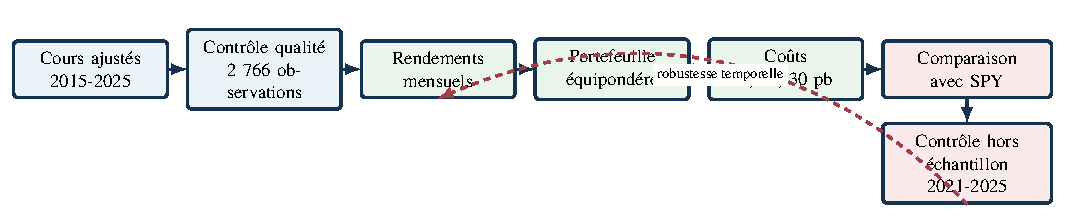
\includegraphics[width=\textwidth]{figures/schemas/protocole_experimental.pdf}
\caption{Déroulement du protocole expérimental et contrôle hors échantillon.}
\label{fig:protocole-experimental}
\end{figure}

\section{Limites de la méthode}

Le benchmark proposé constitue une première validation empirique du socle quantitatif, mais pas une évaluation complète d'un système agentique. Une telle évaluation nécessiterait un univers d'actifs, des données historiques propres, un protocole hors échantillon, une modélisation des coûts et des contraintes de liquidité. L'objectif est donc architectural et méthodologique : identifier les briques pertinentes, analyser leur rôle et proposer une architecture explicable.

Une autre limite concerne l'évolution rapide des dépôts GitHub. Les projets agentiques sont actifs, changent fréquemment d'API et peuvent modifier leur licence ou leur stratégie de maintenance. Toute décision d'adoption doit donc inclure une revue technique datée, une analyse de sécurité des dépendances et une validation juridique de la licence.

% Texte d'exemple du template conservé hors compilation.
